\chapter{Example Programs}
In this Chapter we will present a few small example programs that that illustrate the concepts discussed so far.

\section{Perfect Numbers}
The first example shows the computation of the \blue{perfect} numbers.  A natural number $n$ is a
\href{https://en.wikipedia.org/wiki/Perfect_number}{perfect} number if it is the sum of all its \blue{proper divisors},
where a natural number $t$ is a proper divisor of $n$ if $t$ divides $n$ evenly, i.e. iff
\\[0.2cm]
\hspace*{1.3cm}
$\texttt{mod}\; n\; t = 0$.
\\[0.2cm]
Figure \ref{fig:perfect.hs} on page \pageref{fig:perfect.hs} show a program to compute the list of all perfect
numbers.  The function \texttt{isPerfect} takes a single natural number and checks whether it is perfect, while
the function \texttt{perfect} computes the list of all perfect numbers.

\begin{figure}[!ht]
\centering
\begin{minted}[ frame         = lines, 
                 framesep      = 0.3cm, 
                 firstnumber   = 1,
                 bgcolor       = bg,
                 numbers       = left,
                 numbersep     = -0.2cm,
                 xleftmargin   = 0.8cm,
                 xrightmargin  = 0.8cm,
               ]{python3}
    isPerfect :: Integer -> Bool
    isPerfect n = sum [t | t <- [1.. n-1], mod n t == 0] == n
    
    perfect :: [Integer]
    perfect = [n | n <- [1..], isPerfect n]
\end{minted}
\vspace*{-0.3cm}
\caption{Computing the perfect numbers.}
\label{fig:perfect.hs}
\end{figure}

\section{Computing Word Frequencies}
The following example is inspired by an example from the book
\emph{Thinking Functionally with Haskell} by Richard Bird \cite{bird:2014}.
In \href{https://en.wikipedia.org/wiki/stylometry}{stylometry} one of the tasks is to compute the
relative frequencies of different words occurring in a text.  Stylometry can be used for
\blue{authorship attribution}, compare for example the book \emph{Authorship Attribution} by Patrick
Juola \cite{juola:2008}.  Figure \ref{fig:common-words.hs} on page \pageref{fig:common-words.hs}
shows a program that reads a file, in our case this file contains the text of the book \emph{Moby Dick}
by Herman Melville \cite{melville:1851} and then computes the frequencies of the hundred most common words.

\noindent
Before we can discuss the program from Figure \ref{fig:common-words.hs} we need to discuss some library
functions that we will use.
\begin{enumerate}[(a)]  
\item The \texttt{break} function in Haskell is a higher-order function from the \texttt{Prelude} module that
      is used to split a list into two parts based on a predicate. 
      The type signature of \texttt{break} is:
      \\[0.2cm]
      \hspace*{1.3cm}
      \texttt{break :: (a -> Bool) -> [a] -> ([a], [a])}
      \\[0.2cm]
      Therefore a call of this function has the form
      \\[0.2cm]
      \hspace*{1.3cm}
      \texttt{break p xs}
      \begin{itemize}
      \item The first argument \texttt{p} has type \texttt{(a -> Bool)}.  It is a \textbf{predicate} that
            determines where the list should be split. 
      \item The second argument \texttt{xs} is a list of elements of some generic type \texttt{[a]} that is to
            be split in two parts.
      \item The function satisfies the following specification:
            \begin{lstlisting}[style=haskellstyle, language=Haskell]
  break p xs = (first, second)
      where
          first = [ x | x <- xs, not (p x) ]
          first + second == xs
            \end{lstlisting}
            The return value is a pair.  The \texttt{first} component of this pair is the list of all elements
            \texttt{x} of the list \texttt{xs} that do not satisfy the predicate \texttt{p}.  The
            \texttt{second} component contains the remaining elements of \texttt{xs}.
    \end{itemize}
    For example, we have
    \\[0.2cm]
    \hspace*{1.3cm}
    \texttt{break (> 3) [1, 2, 3, 4, 5] = ([1, 2, 3], [4, 5])}
    \\[0.2cm]
    The function \texttt{break} scans the list from left to right.  It collects elements into the first list
    until the predicate function returns \texttt{True}.  The second list starts from the first element where
    the predicate \texttt{p} is satisfied.  The function \texttt{break} can be implemented as follows:
\begin{lstlisting}[style=haskellstyle, language=Haskell]
break _ [] = ([], [])  -- Base case: Empty list returns two empty lists
break p (x:xs)
    | p x       = ([], x:xs) 
    | otherwise = (x:ys, zs) 
    where (ys, zs) = break p xs
\end{lstlisting}
\item The function \texttt{sort} is part of the \texttt{Data.List} module in Haskell. It is used to sort a list
      in ascending order based on the default ordering of its elements.  It has the following type signature:
      \\[0.2cm]
      \hspace*{1.3cm}
      \texttt{sort ::\;(Ord a) => [a] -> [a]}
      \\[0.2cm]
      Given a list \texttt{xs} the expression \texttt{sort xs} returns the list \texttt{xs} sorted in ascending
      order.
    
      The function requires that the elements of the list belong to the \texttt{Ord} type class (i.e., they must
      support comparison operations).  The implementation in \texttt{Data.List} is using the
      \href{https://en.wikipedia.org/wiki/Merge_sort}{merge sort} algorithm.
\item The function \texttt{words} is part of the \texttt{Data.List} module in Haskell. It is used to split a
      string into a list of words, where words are defined as contiguous sequences of non-whitespace characters. 
      It has the following type signature:
      \\[0.2cm]
      \hspace*{1.3cm}
      \texttt{words :: String -> [String]}
      \\[0.2cm]
      Given a string \texttt{s}, the expression \texttt{words s} breaks \texttt{s} into a list of words, using
      whitespace as the delimiter.  Consecutive whitespace characters are treated as a single separator,
      meaning that empty strings between spaces are ignored.  Leading and trailing whitespace is also ignored.
      The following examples show the behaviour of the function \texttt{words}:
      \begin{itemize}
      \item \texttt{words "Hello, world!" = ["Hello,","world!"]}
      \item \texttt{words "Martin Müller-Lüdenscheid" = ["Martin","Müller-Lüdenscheid"]}
      \end{itemize}
      Note that punctuation marks like ``\texttt{,}'' or ``\texttt{!}'' are not separated from other letters.

      A simple way to implement \texttt{words} recursively is as follows:
      \begin{lstlisting}[style=haskellstyle, language=Haskell]
import Data.Char (isSpace)
words :: String -> [String]
words [] = []  -- Base case: an empty string results in an empty list
words s  = let s' = dropWhile isSpace s  -- drop leading whitespace
           in case s' of
               [] -> []  
               _  -> let (word, rest) = break isSpace s'  
                     in word : words rest  
\end{lstlisting}
      
\item The function \texttt{isAlpha} has type
      \\[0.2cm]
      \hspace*{1.3cm}
      \texttt{isAlpha ::\;Char -> Bool}
      \\[0.2cm]
      and checks, whether the given character is an \blue{alphabetic} Unicode character, i.e.~for a
      character \texttt{c} the call
      \\[0.2cm]
      \hspace*{1.3cm}
      \texttt{isAlpha c}
      \\[0.2cm]
      returns \texttt{True} if \texttt{c} is either one of the lower case letters \texttt{'a'}, $\cdots$,
      \texttt{'z'}, or of the upper case letters \texttt{'A'}, $\cdots$, \texttt{'Z'}, or a
      unicode letter from another script, like, e.g.~the Greek letter $\alpha$.            
\item The function \texttt{toLower} has the following type signature:
      \\[0.2cm]
      \hspace*{1.3cm}
      \texttt{toLower :: Char -> Char}
      \\[0.2cm]
      For a letter \texttt{c}, the expression 
      \\[0.2cm]
      \hspace*{1.3cm}
      \texttt{toLower c}
      \\[0.2cm]
      returns the lower case version of the letter \texttt{c}.  For example,
      \\[0.2cm]
      \hspace*{1.3cm}
      \texttt{toLower 'A' = 'a'} \quad and \quad \texttt{toLower 'b' = 'b'}.
\item The function \texttt{concatMap} has the type
      \\[0.2cm]
      \hspace*{1.3cm}
      \texttt{concatMap ::\;(a -> [b]) -> [a] -> [b]}
      \\[0.2cm]
      Thus, \texttt{concatMap} takes two arguments:
      \begin{itemize}
      \item A function of type \texttt{a -> [b]}, which maps each element of type \texttt{a} to a list of elements
            of type \texttt{b}. 
      \item A list of type \texttt{a}, which serves as the input to be processed.
      \end{itemize}
      The result is a single list of type \texttt{b} obtained by applying the function to each element of the
      input list and then concatenating the resulting lists. 

      The function \texttt{concatMap} can be understood as the composition of \texttt{map} and \texttt{concat}:
      \begin{itemize}
      \item \texttt{map} applies the given function to each element of the input list, producing a list of lists:
            \texttt{[a] -> [[b]]}. 
      \item \texttt{concat} then flattens this list of lists into a single list: \texttt{[[b]] -> [b]}.
      \end{itemize}
      Formally, we can express this as:
      \\[0.2cm]
      \hspace*{1.3cm}
      \texttt{concatMap f xs = concat (map f xs)}
      \\[0.2cm]
      where:
      \begin{itemize}
      \item \texttt{f} is the function of type \texttt{a -> [b]},
      \item \texttt{xs} is the input list of type \texttt{[a]}.
      \end{itemize}
      The following example shows \texttt{concatMap} at work:
      \\[0.2cm]
      \hspace*{1.3cm}
      \texttt{concatMap (\textbackslash x -> [x, x+1]) [1, 3, 5]}
      \begin{itemize}
      \item The function \texttt{\symbol{92}x -> [x, x+1]} maps each element \texttt{x} to the list \texttt{[x, x+1]}.
      \item Applying \texttt{map} yields the list of lists  \texttt{[[1, 2], [3, 4], [5, 6]]}.
      \item Applying \texttt{concat} flattens this to \texttt{[1, 2, 3, 4, 5, 6]}.
      \end{itemize}
      Thus, the result is the list
      \\[0.2cm]
      \hspace*{1.3cm}
      \texttt{[1, 2, 3, 4, 5, 6]}.   
\end{enumerate}

\begin{figure}[!ht]
\centering
\begin{minted}[ frame         = lines, 
                framesep      = 0.3cm, 
                firstnumber   = 1,
                bgcolor       = bg,
                numbers       = left,
                numbersep     = -0.2cm,
                xleftmargin   = 0.0cm,
                xrightmargin  = 0.0cm,
              ]{haskell}
    import Data.List (sort, words)
    import Data.Char (isAlpha, toLower)
    
    type Text = [Char]
    
    countRuns :: Eq a => [a] -> [(Int, a)]
    countRuns [] = []
    countRuns (x:xs) =
        let (run, rest) = break (/= x) xs
        in (1 + length run, x) : countRuns rest
    
    frequency :: Int -> Int -> Double
    frequency c n = fromIntegral c / fromIntegral n 
    
    divide :: Int -> [(Int, a)] -> [(Double, a)]
    divide n ps = [(frequency c n, x) | (c, x) <- ps]
    
    myWords :: String -> [String]
    myWords = map (filter isAlpha) . words
    
    showPair :: (Double, String) -> String 
    showPair (f, w) = w ++ ": " ++ show f ++ "\n"
    
    comnWrds :: Int -> Text -> String
    comnWrds n b = concatMap showPair $
                   divide nw . take n . reverse . sort . countRuns . sort $
                   aw
      where
        aw = (myWords . map toLower) b
        nw = length aw
                     
    readBook :: FilePath -> IO String
    readBook filename = readFile filename
    
    main :: IO ()
    main = do
        contents <- readBook "moby-dick.txt"
        putStrLn $ comnWrds 100 contents
\end{minted} 
\vspace*{-0.3cm}
\caption{Finding the most common words, \texttt{part \texttt{I}}.}
\label{fig:common-words.hs}
\end{figure} %$


We proceed to discuss the program that is shown in Figure \ref{fig:common-words.hs} on page
\pageref{fig:common-words.hs}. 
\begin{enumerate}
\item In line 1, we import the functions \texttt{sort} and \texttt{words} from the module \texttt{Data.List}. 
\item Similarly, we import \texttt{isAlpha} and \texttt{toLower} in line 2.
\item The function \texttt{countRuns} takes a sorted list of elements of type \texttt{a}
      and returns a list of pairs.  Each pair consists of a unique element from the input list
      and the count of its consecutive occurrences (runs).
      For example, we have:
      \\[0.2cm]
      \hspace*{0.8cm}
      \texttt{countRuns ['a','a','a','a','b','c','c'] = [(4,'a'),(1,'b'),(2,'c')]}
      \\[0.2cm]
      The implementation is recursive.  If the given list is non-empty and therefore has the form
      \texttt{x:xs}, we first check how often the element \texttt{x} occurs at the beginning of the list
      \texttt{xs} by breaking \texttt{xs} into two sublists:
      \begin{itemize}
      \item \texttt{run} is the longest prefix of the list \texttt{xs} that only contains the element
            \texttt{x}.
      \item \texttt{rest} is the remainder of the list \texttt{xs} after removing all occurrences of the
            element \texttt{x} from the beginning of the list \texttt{xs}.    
      \end{itemize}
      Then the element \texttt{x} occurs \texttt{1 + length run} times in the list \texttt{x:xs} because it
      occurs \texttt{length run} times in \texttt{xs} and it also is the first element of the list \texttt{x:xs}.
      Furthermore, we have to call \texttt{countRuns} recursively on the \texttt{rest} list.
\item The function \texttt{frequency} takes two natural numbers as its input.
      \begin{itemize}
      \item \texttt{c} is the number of occurrences of a given word, while
      \item \texttt{n} is the total number of words.
      \end{itemize}
      The function computes the fraction \texttt{c/n}.  It makes use of the function
      \\[0.2cm]
      \hspace*{1.3cm}
      \texttt{fromIntegral ::\;Int -> Double}
      \\[0.2cm]
      that transforms a natural number into a floating point number.  This is necessary, because division is
      only defined for floating point numbers.
\item The function \texttt{divide} is called with two arguments:
      \\[0.2cm]
      \hspace*{1.3cm}
      \texttt{divide n ps}
      \\[0.2cm]
      Here, \texttt{n} is the total number of words, while \texttt{ps} is a list of pairs of the form
      \texttt{(c, w)} where \texttt{w} is a word and \texttt{c} is the number of occurrences of this word in a
      given text.  It converts the number of occurrences into frequencies by dividing the count \texttt{c} by
      the total number of words.     
\item When we use the function \texttt{words}, the resulting words will contain punctuation symbols.  For
      example, we have
      \\[0.2cm]
      \hspace*{1.3cm}
      \texttt{words "Hello, world!" == ["Hello," ,"world!"]}
      \\[0.2cm]
      This is not what we want.  The function \texttt{myWords} takes a string, extracts the words and finally removes
      all symbols from these words that are not alphabetical characters.
\item The function \texttt{showPair} is only used to format the output.  It takes a pair of the form
      $(f, w)$ where $w$ is a word and $f$ is the frequency of this words.  It returns a string of the form 
      $\texttt{\symbol{34}}w\mathtt{:}\; f\texttt{\symbol{92}n\symbol{34}}$, where
      \texttt{\symbol{92}n\symbol{34}} is a newline symbol.
\item The function \texttt{comnWrds} is the star of the show and does the main work of extraction the word and
      computing their frequencies. The function receives two arguments
      \begin{enumerate}[(a)]
      \item \texttt{n} is the number of words that should be returned.
      \item \texttt{b} is a string representing a book.
      \end{enumerate}
      The task of the function is to return the \texttt{n} most common word from the book \texttt{b}.

      The implementation works by chaining a number of different functions together in a pipeline.
      \begin{enumerate}[(a)]
      \item The variable \texttt{aw} (short for \underline{\texttt{a}}ll \underline{\texttt{w}}ords) is a list
            containing all words.  Note that we first transform all characters in the string \texttt{b} to
            lower case before we extract the list of words.  This way, the strings ``The''  and ``the''
            represent the same word.
      \item The variable \texttt{nw}  (short for \underline{\texttt{n}}umber of \underline{\texttt{w}}ords)
            stores the number of all different words that have been found.
      \item Next, the words are sorted using the function \texttt{sort}.  This way, the same words are grouped
            together and hence it is easy to count how often each word occurs.
      \item The function \texttt{countRuns} counts the frequency of each words.  It transforms the sorted list
            of words into a list of pairs of the form
            \\[0.2cm]
            \hspace*{1.3cm}
            \texttt{[(1, "abasement"), (1, "abandonedly"), ... (981, "of"), (1073, "the"), ...]}
            \\[0.2cm]
            In these pairs, the first component is the number of occurrences of the corresponding word.
            This list is the sorted ascendingly according to the number of occurrences.  
      \item Since we want the most frequent words at the beginning, this list is reversed.
      \item Then we \texttt{take} the first \texttt{n} pairs from this list.
      \item The function \texttt{divide} turns a pair of the form
            \\[0.2cm]
            \hspace*{1.3cm}
            $(c, w)$
            \\[0.2cm]
            where $w$ is a word and $c$ is the number of occurrences of this word into a pair of the form
            \\[0.2cm]
            \hspace*{1.3cm}
            $(f, w)$
            \\[0.2cm]
            where $f$ is the frequency of the word.  This is done by dividing $c$ by the total number of all
            words \texttt{nw}.
      \item Finally, the function \texttt{concatMap} turns the list of pairs into a string with the help of the
            function \texttt{showPair}.
      \end{enumerate}      
\end{enumerate}

 
\section{The Wolf, the Goat, and the Cabbage}
Next,  we show how to solve logical puzzles with \textsl{Haskell}.  The puzzle we
want to solve is known as the  
\href{https://en.wikipedia.org/wiki/Wolf,_goat_and_cabbage_problem}{wolf, goat, and cabbage problem}:  
\vspace*{0.3cm}

\begin{minipage}[c]{15cm}
{\sl
An farmer has to sell a wolf, a goat, and a cabbage on a market place.  In order to
reach the market place, she has to cross a river.  The boat that she can use is so small that it can
only accommodate either the goat, the wolf, or the cabbage in addition to the farmer.
Now if the farmer leaves the wolf alone with the goat, the wolf will eat the goat.
If, instead, the farmer leaves the goat with the cabbage, the goat will eat the cabbage.
Is it possible for the farmer to develop a schedule that allows her to cross the river
without either the goat or the cabbage being eaten?
}
\end{minipage}
\vspace*{0.3cm}

\noindent
We will solve this problem by formulating it as a \blue{search problem}.  This search problem is then solved
via \href{https://en.wikipedia.org/wiki/Breadth-first_search}{breadth first search}.

\begin{Definition}[Search Problem]
  A \blue{search problem} \index{search problem} is a 4-tuple of the form
  \\[0.2cm]
  \hspace*{1.3cm}
  $\mathcal{P} = \langle Q,\;R,\; \mathtt{start},\; \mathtt{goal}\rangle$
  \\[0.2cm]
  where
  \begin{enumerate}[(a)]
  \item $Q$ is the set of \blue{states}, also known as the \blue{state space}.
        \index{state}
  \item $R$ is a binary relation on $Q$, i.e.~we have $R \subseteq Q \times Q$.

        If $\langle x, y \rangle \in Q$, then there is a direct connection between the states $x$ and $y$,
        that is we can move in one step from the state $x$ to the state $y$.
  \item \texttt{start} is the \blue{start state}, hence $\mathtt{start} \in Q$.
  \item \texttt{goal} is the \blue{goal state}, hence $\mathtt{goal} \in Q$.    
  \end{enumerate}
  A \blue{path} \index{path} is a list $[s_1, \cdots, s_n]$ such that $\langle s_{i}, s_{i+1} \rangle \in R$
  for all $i \in \{1,\cdots,n-1\}$.  The \blue{length} of this path is defined as the length of this list minus
  1, i.e.~the path $[s_1, \cdots, s_n]$ has length $n-1$.  The reason for defining the length of this path as
  $n-1$ and not $n$ is that the path consists of $n-1$ \blue{edges} \index{edge} of the form $\langle s_i, s_{i+1} \rangle$ where
  $i \in \{1, \cdots, n-1\}$.
  A path $[s_1, \cdots, s_n]$ is a \blue{solution} to the search problem $\mathcal{P}$ iff the following conditions are satisfied:
  \begin{enumerate}
  \item $s_1 = \mathtt{start}$, i.e.~the first element of the path is the start state.
  \item $s_n = \mathtt{goal}$, i.e.~the last element of the path is the goal state. \eox
  \end{enumerate}
\end{Definition}

\noindent
We will model the wolf, goat, and cabbage problem as a search problem.
To this end we define the set
\\[0.2cm]
\hspace*{1.3cm} 
$\texttt{all} := \{ \squote{farmer},\; \squote{wolf},\; \squote{goat},\; \squote{cabbage} \}$.
\\[0.2cm]
Every state will be represented as a subset \texttt{s} of the set \texttt{all}.  The idea is that the set \texttt{s}
specifies those objects that are on the left side of the river.  We assume that initially the farmer
is on the left side of the river. 
Therefore, the set of all possible states can be defined as the set
\\[0.2cm]
\hspace*{1.3cm}
$Q := \bigl\{ s \mid s \in 2^{\mathtt{all}} \wedge \neg \mathtt{problem}(s) \wedge \neg \mathtt{problem}(\mathtt{all} \backslash s) \bigl\}$
\\[0.2cm]
Here, we have used the procedure \texttt{problem} to check whether a given state \texttt{s} has a
\blue{problem}, meaning that either the wolf can eat the goat or the goat can eat the cabbage. 
Note that since \texttt{s} is the set of objects on the left side, the expression $\texttt{all} \backslash s$
computes the set of objects on the right side of the river.

We implement a function \texttt{problem} that takes a set \texttt{s} of items as input and checks whether there
is a problem.  A state \texttt{s} of objects has a problem if both of the following conditions are satisfied:
\begin{enumerate}
\item The farmer is not an element of the set \texttt{s} and
\item either \texttt{s} contains both the goat and the cabbage or \texttt{s} contains both the wolf and the goat.
\end{enumerate}
Therefore, we can implement the function \texttt{problem} in \textsl{Haskell} as follows:

\begin{minted}[ frame         = lines, 
                 framesep      = 0.3cm, 
                 firstnumber   = 1,
                 bgcolor       = white,
                 numbers       = left,
                 numbersep     = -0.2cm,
                 xleftmargin   = 0.0cm,
                 xrightmargin  = 0.0cm,
               ]{haskell}
    problem :: Set String -> Bool
    problem s = "farmer" ∉ s &&
                (("goat" ∈ s && "cabbage" ∈ s) ||  -- goat eats cabbage
                 ("wolf" ∈ s && "goat"    ∈ s))    -- wolf eats goat
\end{minted}
We proceed to compute the relation $R$ that contains all possible transitions between
different states.  We will compute $R$ using the formula:
\\[0.2cm]
\hspace*{1.3cm}
$R := R_1 \cup R_2$
\\[0.2cm]
Here $R_1$ describes the transitions that result from the farmer crossing the river from left
to right, while $R_2$ describes the transitions that result from the farmer crossing the river
from right to left.  Mathematically, we can define the relation $R_1$ as follows:
\\[0.2cm]
\hspace*{1.3cm}
$R_1 := \bigl\{ \langle s, s \backslash b \rangle \mid s \in Q \wedge b \in 2^s \wedge s \backslash b \in Q \wedge
                \squote{farmer} \in b \wedge \mathtt{card}(b) \leq 2 \bigr\}$
\\[0.2cm]
Let us explain this definition in detail:
\begin{enumerate}
\item Initially, $s$ is the set of objects on the left side of the river.  Hence, $s$
      is an element of the set of all states that we have defined as $Q$.
\item $b$ is the set of objects that are put into the boat and that do cross the river.  Of
      course, for an object to go into the boat is has to be on the left side of the river to begin
      with.  Therefore, $b$ is a subset of $s$ and hence an element of the power set
      of $s$. 
\item Then  $s \backslash b$ is the set of objects that are left on the left side of the river after
      the boat has crossedthe river.  Of course, the new state $s \backslash b$ has to be a state that does not
      have a problem.  Therefore, we check that $s \backslash b$ is an element of the set of states $Q$.
\item Furthermore, the farmer has to be in the boat.  This explains the condition 
      \\[0.2cm]
      \hspace*{1.3cm}
      $\squote{farmer} \in b$.
\item Finally, the boat can only have two passengers.  Therefore, we have added the condition
      \\[0.2cm]
      \hspace*{1.3cm}
      \texttt{\texttt{card}(b) <= 2}.
      \\[0.2cm]
      Here, the function \texttt{card} computes the \emph{cardinality} of the set $b$, i.e.~it computes the
      number of elements of $b$.
\end{enumerate}
Next, we have to define the relation $R_2$.  However, as crossing the river from right to left
is just the reverse of crossing the river from left to right, $R_2$ is just the inverse of
$R_1$.   Hence we define:
\\[0.2cm]
\hspace*{1.3cm}
$R_2  := \bigl\{ \langle y, x \rangle \mid \langle x, y \rangle \in R_1 \bigr\}$
\\[0.2cm]
Finally, the start state has all objects on the left side.  Therefore, we have
\\[0.2cm]
\hspace*{1.3cm}
$\texttt{start} := \texttt{all}$
\\[0.2cm]
In the end, all objects have to be on the right side of the river.  That means that nothing is left
on the left side.  Therefore, we define
\\[0.2cm]
\hspace*{1.3cm}
$\texttt{goal} := \{\}$
\\[0.2cm]
Figure \ref{fig:wolf-goat-cabbage.hs} on page \pageref{fig:wolf-goat-cabbage.hs} shows a \textsl{Haskell} program that 
formulates the wolf, goat, and cabbage problem as a search problem.
We discuss this program line by line:

\begin{figure}[!ht]
\centering
\begin{minted}[ frame         = lines, 
                 framesep      = 0.3cm, 
                 firstnumber   = 1,
                 bgcolor       = white,
                 numbers       = left,
                 numbersep     = -0.2cm,
                 xleftmargin   = 0.0cm,
                 xrightmargin  = 0.0cm,
               ]{haskell}
    {-# LANGUAGE UnicodeSyntax #-}
    import Data.Set (Set, (\\), fromList, toList, filter)
    import Bfs (search)
    import SetUtils (power, (∈), (∉))
      
    problem :: Set String → Bool
    problem s = "farmer" ∉ s &&
                (("goat" ∈ s && "cabbage" ∈ s) ||  -- goat eats cabbage
                 ("wolf" ∈ s && "goat"    ∈ s))    -- wolf eats goat
    
    allItems :: Set String
    allItems = fromList ["farmer", "wolf", "goat", "cabbage"]
    
    noProblem :: Set String → Bool
    noProblem s = not (problem s) && not (problem $ allItems \\ s)
    
    states :: Set (Set String)
    states = Data.Set.filter noProblem (power allItems)
    
    r1 :: [(Set String, Set String)]
    r1 = [ (s, s \\ b) | s ← toList states,
                         b ← toList $ power s, s \\ b ∈ states,
                         "farmer" ∈ b, length b <= 2
         ]
    
    r2 :: [(Set String, Set String)]
    r2 = [ (s1, s2) | (s2, s1) ← r1 ]
    
    r :: [(Set String, Set String)]
    r = r1 ++ r2
    
    start :: Set String
    start = allItems
    
    goal :: Set String
    goal = fromList []
    
    main :: IO ()
    main = mapM_ (putStrLn . show) $ head $ search r start goal 
\end{minted}
\vspace*{-0.3cm}
\caption{The wolf, the goat, and the cabbage.}
\label{fig:wolf-goat-cabbage.hs}
\end{figure}

\begin{enumerate}
\item In the first line we activate the \blue{Unicode syntax language extension}.  This language extension enables us
      to use Unicode characters as operator symbols.

      Normally, every text that is enclosed in the strings ``\texttt{\{-}'' and ``\texttt{-\}}'' is considered a comment.
      However, there is one exception:  If a multiline comment starts as ``\texttt{\{-\# }'' and ends
      with ``\texttt{\#-\}}, then the comment is considered a \blue{pragma}. A pragma can be used to activate a
      \blue{language extension}. 
\item In line 2 we import a number of items from the module \texttt{Data.Set}.
      \begin{enumerate}
      \item \texttt{Set} is the type of sets.
      \item The operator \texttt{(\symbol{92}\symbol{92})} is used to build the difference of two sets, i.e.~if
            $a$ and $b$ are sets, then
            \\[0.2cm]
            \hspace*{1.3cm}
            $a \;\mathtt{\symbol{92}\symbol{92}}\; b := \{\, x \in a \mid x \not\in b \,\}$.
      \item The function \texttt{fromList} has type signature
            \\[0.2cm]
            \hspace*{1.3cm}
            \texttt{fromList ::\;Ord a => [a] -> Set a}.
            \\[0.2cm]
            The expression \texttt{fromList l} takes a list \texttt{l} of elements that can be compared
            and returns a set containing the elements of \texttt{l}.  We have to require that the type $a$
            belongs to the type class \texttt{Ord} because in Haskell sets are implemented as
            \href{https://en.wikipedia.org/wiki/Binary_search_tree}{ordered binary search trees} and hence the
            elements of a set need to be comparable. 
      \item The function \texttt{toList} has type signature
            \\[0.2cm]
            \hspace*{1.3cm}
            \texttt{toList ::\;Set a -> [a]}.
            \\[0.2cm]
            The expression \texttt{toList s} takes a set \texttt{s} of elements 
            and returns a list containing the elements of \texttt{s}.
      \item The function \texttt{Data.Set.filter} has type signature
            \\[0.2cm]
            \hspace*{1.3cm}
            \texttt{Data.Set.filter ::\;(a -> Bool) -> Set a -> Set a}.
            \\[0.2cm]
            The expression \texttt{Data.Set.filter p s} takes a predicate \texttt{p} and a set \texttt{s}.
            It returns a new set containing those elements \texttt{x} of \texttt{s} such that \texttt{p x} is
            \texttt{True}:
            \\[0.2cm]
            \hspace*{1.3cm}
            \texttt{Data.Set.filter p s = \{ x $\in$ s | p x \}}
            \\[0.2cm]
            Note that we have to qualify the function name \texttt{filter} as \texttt{Data.Set.filter} in order
            to distinguish it from the predefined function \texttt{filter} that has the type signature
            \\[0.2cm]
            \hspace*{1.3cm}
            \texttt{Data.Set.filter ::\;(a -> Bool) -> [a] -> [a]}.
      \end{enumerate}
      \item Line 3 imports the module \texttt{Bfs} which implements
            \href{https://en.wikipedia.org/wiki/Breadth-first_search}{breadth-first search}.  We import the
            function \texttt{search} from this module, which has the following type signature:
            \\[0.2cm]
            \hspace*{1.3cm}
            \texttt{search ::\;Ord a => [(a, a)] -> a -> a -> [Bfs.Path a]}
            \\[0.2cm]
            The function \texttt{search} is called as follows:
            \\[0.2cm]
            \hspace*{1.3cm}
            \texttt{search r s g}
            \\[0.2cm]
            Here \texttt{r} is a binary relation on some set of states \texttt{q}, i.e.~we have
            $\texttt{r} \in \texttt{q} \times \texttt{q}$. The arguments \texttt{s} and \texttt{g} are elements
            of \texttt{q} and the function returns a list of all shortest paths leading from the state
            \texttt{s} (\underline{s}tart) to the state \texttt{g} (\underline{g}oal).

            The module \texttt{Bfs} is shown in Figure \ref{fig:Bfs.hs} on page
            \pageref{fig:Bfs.hs}. 
      \item In line 4 we import the module \texttt{SetUtils}.  This module provides a number of functions and
            operators that are useful when working with sets.
            \begin{enumerate}
            \item The function \texttt{power} has the type signature
                  \\[0.2cm]
                  \hspace*{1.3cm}
                  \texttt{power :: Ord a => Set a -> Set (Set a)}
                  \\[0.2cm]
                  Given a set \texttt{s} the expression \texttt{power s} computes the set of all subsets of
                  \texttt{s}, i.e.~we have
                  \\[-0.2cm]
                  \hspace*{1.3cm}
                  \texttt{power s = \{ a \;|\; a $\subseteq$ s \}}.
                  \\[0.2cm]
                  For exampe, we have:
                  \\[0.2cm]
                  \hspace*{1.3cm}
                  \texttt{power \{1, 2\} = \{\{\}, \{1\}, \{1,2\}, \{2\}\}}
            \item The binary operator ``$\in$'' has the type signature
                  \\[0.2cm]
                  \hspace*{1.3cm}
                  \texttt{(∈) :: Ord a => a -> Set a -> Bool}
                  \\[0.2cm]
                  The expression $x \in s$ yields \texttt{True} if and only if $x$ is an element from the set $s$.
            \item The binary operator ``$\not\in$'' is the negation of the operator ``$\in$''.
            \end{enumerate}
            The module \texttt{SetUtils} is shown in Figure \ref{fig:SetUtils.hs} on page \pageref{fig:SetUtils.hs}.
      \item Line 6--9 define the function \texttt{problem}.  This function takes a state, i.e.~a set of the
            items on a shore and returns \texttt{True} if there would be a problem on that shore.
      \item Line 12 defines the set \texttt{allItems} as
            \\[0.2cm]
            \hspace*{1.3cm}
            $\{ \squote{farmer},\; \squote{wolf},\; \squote{goat},\; \squote{cabbage} \}$.
      \item The function \texttt{noProblem} takes a set \texttt{s} of items as its argument.  This set represents
            the items on the left shore.  It checks that there is neither a problem on the left shore nor on
            the right shore.

            Note that if \texttt{s} is the set of items on the left shore, then
            \texttt{allItems \symbol{92}\symbol{92} s} is the set of items on the right shore.
      \item \texttt{states} is the set of all states of the search problem.   These are those subsets of the
            set \texttt{allItems} such that there is no problem on either shore.
      \item \texttt{r1} is the relation that describes all those transitions from the left shore to the right
            shore that do not lead to a problematic state.  Rather than representing this relation as a set of
            pairs it is represented as a list of pairs because this makes the definition a little bit more convenient.
            \begin{enumerate}[(a)]
            \item \texttt{s} is a state.
            \item \texttt{b} is the set of items that cross the river on the boat.
                  \begin{itemize}
                  \item First of all, \texttt{b} has to be a subset of \texttt{s} because only item on the left
                        shore cross the river from the left to the right.
                  \item The new state is \texttt{s \symbol{92}\symbol{92} b} must not be problematic.
                        Hence it has to be a memeber of \texttt{states}.
                  \item The \squote{farmer} has to be on the boat and there may be at most two items on the boat.
                  \end{itemize}
            \item After the crossing of the river the new state is the set of those items that are left on the
                  left shore \texttt{s \symbol{92}\symbol{92} b}.
            \end{enumerate}
      \item \texttt{r2} is the inverse of the relation \texttt{r1}.
      \item \texttt{r} is the union of the relations \texttt{r1} and \texttt{r2}.
      \item The \texttt{start} state is the state where all items are on the left shore.
      \item The \texttt{goal} state is the state where all items are on the right shore.  Hence nothing is left
            on the left shore.
      \item The expression \texttt{search r start goal} computes the list of all minimal paths from \texttt{start} to
            \texttt{goal} and the function \texttt{head} extracts the first such path.

            This path is a list. The elements of this list are then converted to strings via \texttt{show} and
            printed on separate lines via \texttt{putStrLn}.
      \item The function \texttt{mapM\_} is a variant of the function \texttt{map} that works with functions
            performing \texttt{IO}.
 \end{enumerate}


\begin{figure}[!ht]
\centering
\begin{minted}[ frame         = lines, 
                 framesep      = 0.3cm, 
                 firstnumber   = 1,
                 bgcolor       = white,
                 numbers       = left,
                 numbersep     = -0.2cm,
                 xleftmargin   = -0.3cm,
                 xrightmargin  = 0.0cm,
               ]{python3}
    {-# LANGUAGE UnicodeSyntax #-}
    module Bfs (search) where
    
    import Data.Set (Set)
    import qualified Data.Set as Set
    
    (∪) :: Ord a ⇒ Set a → Set a → Set a
    (∪) = Set.union
    
    (∈) :: (Ord a) ⇒ a → Set a → Bool
    (∈ ) = Set.member
    
    (∉) :: (Ord a) ⇒ a → Set a → Bool
    x ∉ s = not (x ∈ s)
    
    type Path a = [a]
    
    search :: forall a. Ord a ⇒ [(a, a)] → a → a → [Path a]
    search relation start goal = go [[start]] (Set.singleton start)
      where
        go :: [Path a] → Set a → [Path a]
        go [] _ = []
        go paths visited
          | null goalPaths = go newPaths newVisited
          | otherwise = goalPaths
          where
            newPaths = [ path ++ [z] | path ← paths, (y, z) ← relation, 
                                       last path == y, z ∉ visited       ]
            newVisited = visited ∪ Set.fromList [last path | path ← newPaths]
            goalPaths = filter (\p → last p == goal) newPaths
\end{minted}
\vspace*{-0.3cm}
\caption{Breadth First Search.}
\label{fig:Bfs.hs}
\end{figure}
\noindent

\begin{figure}[!ht]
\centering
\begin{minted}[ frame         = lines, 
                framesep      = 0.3cm, 
                firstnumber   = 1,
                bgcolor       = white,
                numbers       = left,
                numbersep     = -0.2cm,
                xleftmargin   = 0.0cm,
                xrightmargin  = 0.0cm,
              ]{haskell}
    {-# LANGUAGE UnicodeSyntax #-}
    module SetUtils (power, (∪), (∩), (∈), (∉), (∅)) where
    
    import Data.Set (Set, (\\), fromList, toList, findMin, insert)
    import qualified Data.Set as Set
    
    -- the empty set
    (∅) :: Ord a ⇒ Set a
    (∅) = fromList []
    
    -- union of sets
    (∪) :: Ord a ⇒ Set a → Set a → Set a
    (∪) = Set.union
    
    -- intersection of sets
    (∩) :: Ord a ⇒ Set a → Set a → Set a
    (∩) = Set.intersection
    
    -- is x an element of s
    (∈) :: (Ord a) ⇒ a → Set a → Bool
    x ∈ s = x `Set.member` s
    
    -- is x not an element of s
    (∉) :: (Ord a) ⇒ a → Set a → Bool
    x ∉ s = not (x ∈ s)
    
    -- compute the power set of the set s
    power :: Ord a ⇒ Set a → Set (Set a)
    power s
      | Set.null s = fromList [ (∅) ]
      | otherwise  = p ∪ Set.map (\x → insert m x) p 
        where m = findMin s
              p = power (s \\ fromList [m])
\end{minted}
\vspace*{-0.3cm}
\caption{The set utilities.}
\label{fig:SetUtils.hs}
\end{figure}


\begin{figure}[h]
  \centering

  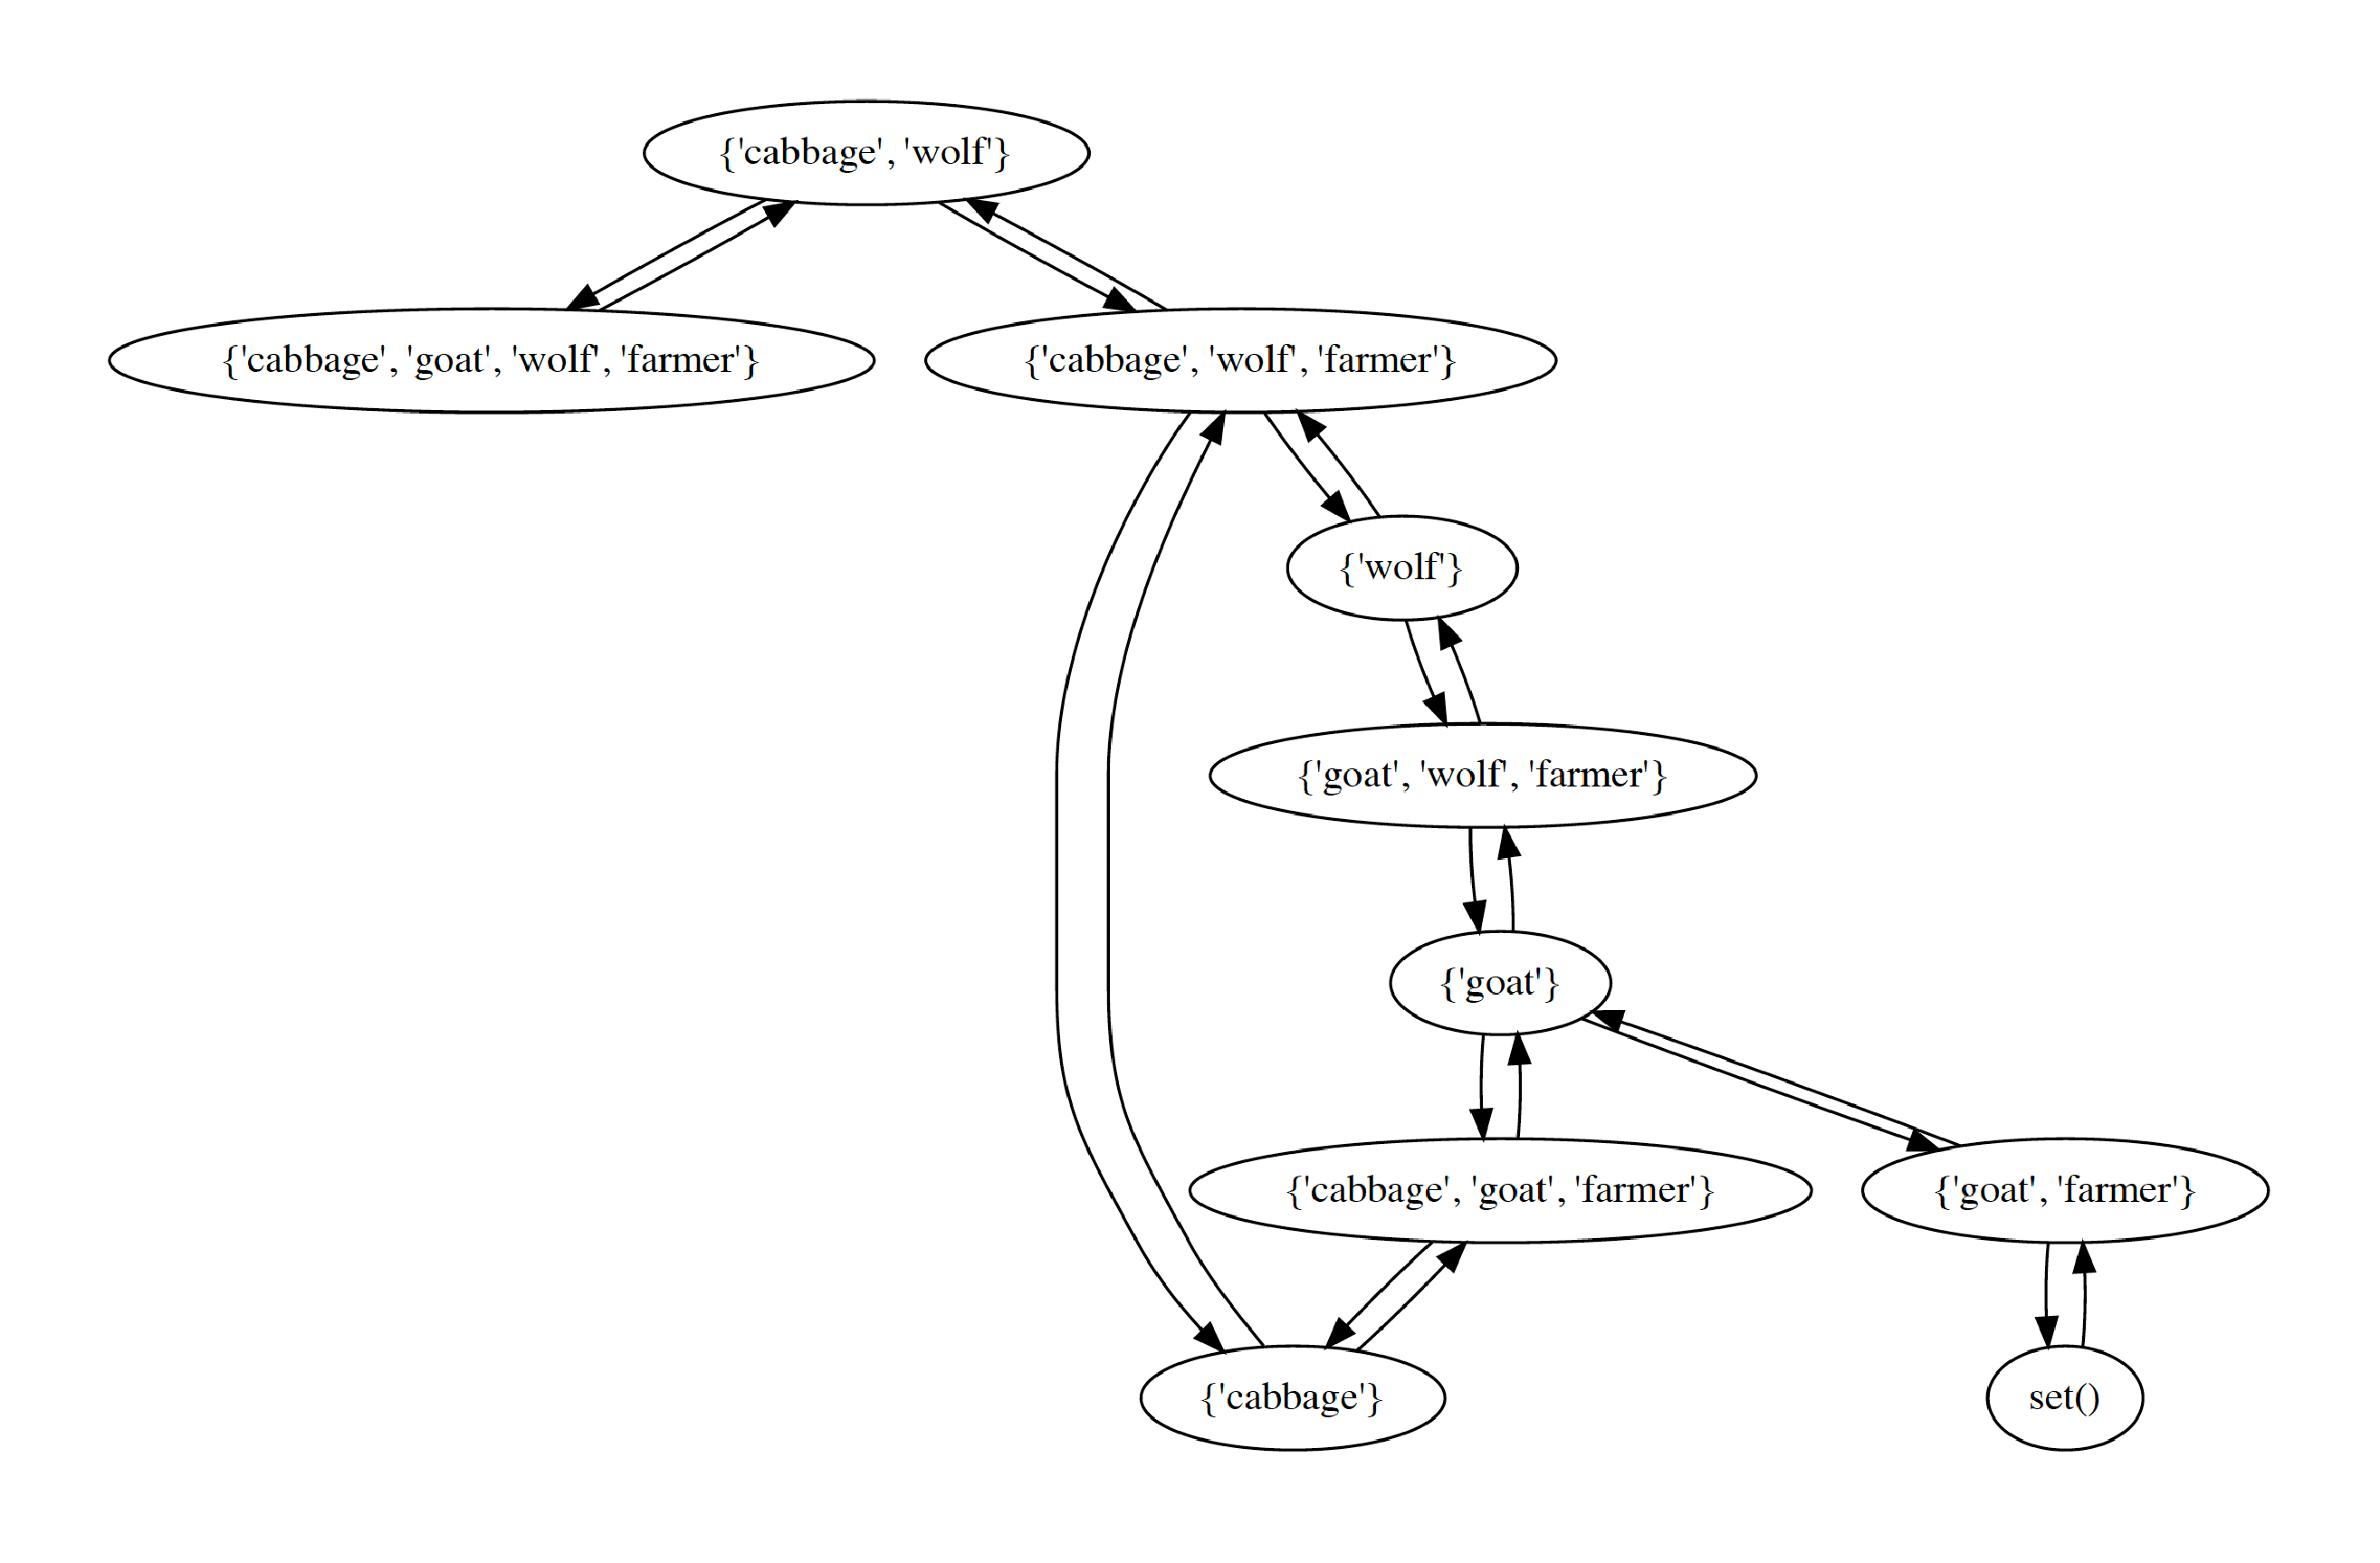
\epsfig{file=Figures/wolf-goat-cabbage, scale=0.4}

  \caption{The relation \texttt{R} shown as a directed graph.}
  \label{fig:wolf-goat-cabbage.pdf}
\end{figure}



\noindent
Figure \ref{fig:wolf-goat-cabbage.pdf} on page \pageref{fig:wolf-goat-cabbage.pdf} displays the relation $R$ graphically.

Figure \ref{fig:wolf-ziege-solution} shows a shedule for solving the puzzle.




\begin{figure}[!ht]
  \centering
\begin{minted}[ frame         = lines, 
                framesep      = 0.3cm, 
                numbers       = left,
                numbersep     = -0.2cm,
                bgcolor       = bg,
                xleftmargin   = 0.8cm,
                xrightmargin  = 0.8cm,
              ]{python3}
    {'cabbage', 'farmer', 'goat', 'wolf'}                                 {}
                             >>>> {'farmer', 'goat'} >>>> 
    {'cabbage', 'wolf'}                                   {'farmer', 'goat'}
                             <<<< {'farmer'} <<<< 
    {'cabbage', 'farmer', 'wolf'}                                   {'goat'}
                             >>>> {'farmer', 'wolf'} >>>> 
    {'cabbage'}                                   {'farmer', 'goat', 'wolf'}
                             <<<< {'farmer', 'goat'} <<<< 
    {'cabbage', 'farmer', 'goat'}                                   {'wolf'}
                             >>>> {'cabbage', 'farmer'} >>>> 
    {'goat'}                                   {'cabbage', 'farmer', 'wolf'}
                             <<<< {'farmer'} <<<< 
    {'farmer', 'goat'}                                   {'cabbage', 'wolf'}
                             >>>> {'farmer', 'goat'} >>>> 
    {}                                 {'cabbage', 'farmer', 'goat', 'wolf'}
\end{minted} 
\vspace*{-0.3cm}
\caption{A schedule for the farmer.}  
\label{fig:wolf-ziege-solution}
\end{figure}

\FloatBarrier

\section{Symbolic Differentiation}
Figure \ref{fig:differentiate.hs} onm page \pageref{fig:differentiate.hs}
shows a package that implements a crude form of symbolic differentiation.  For example, when given the
expression $x^x$ this program is able to show that 
\\[0.2cm]
\hspace*{1.3cm}
$\frac{\,\mathrm{d}\;\;\,}{\,\mathrm{d}\,x} x^x = x^x \cdot \bigl( \ln(x) + 1 \bigr)$.
\\[0.2cm]
We discuss this program line by line.

\begin{figure}[!ht]
\centering
\begin{minted}[ frame         = lines, 
                 framesep      = 0.3cm, 
                 firstnumber   = 1,
                 bgcolor       = white,
                 numbers       = left,
                 numbersep     = -0.2cm,
                 xleftmargin   = 0.0cm,
                 xrightmargin  = 0.0cm,
               ]{haskell}
    {-# LANGUAGE UnicodeSyntax #-}
    data Expr = Add Expr Expr
              | Sub Expr Expr
              | Mul Expr Expr
              | Div Expr Expr
              | Pow Expr Expr
              | Exp Expr
              | Ln  Expr
              | Var Char
              | Num Double
    
    instance Show Expr where
      show :: Expr → String          
      show (Add x y) = "(" ++ (show x) ++ "+" ++ (show y) ++ ")"
      show (Sub x y) = "(" ++ (show x) ++ "-" ++ (show y) ++ ")"
      show (Mul x y) = "(" ++ (show x) ++ "*" ++ (show y) ++ ")"
      show (Div x y) = "(" ++ (show x) ++ "/" ++ (show y) ++ ")"
      show (Pow x y) = "(" ++ (show x) ++ "^" ++ (show y) ++ ")"
      show (Exp x)   = "exp(" ++ show(x) ++ ")"
      show (Ln  x)   = "ln("  ++ show(x) ++ ")"
      show (Var c)   = [c]
      show (Num x)   = show x
    
    diff :: Expr → Char → Expr
    diff (Add f g) x = Add fs gs
      where fs = diff f x; gs = diff g x
    diff (Sub f g) x = Sub fs gs
      where fs = diff f x; gs = diff g x
    diff (Mul f g) x = Add (Mul fs g) (Mul f gs)
      where fs = diff f x; gs = diff g x
    diff (Div f g) x = Div (Sub (Mul fs g) (Mul f gs)) (Mul g g)
      where fs = diff f x; gs = diff g x
    diff (Pow f g) x = diff (Exp (Mul g (Ln f))) x 
    diff (Exp f) x = Mul (Exp f) fs
      where fs = diff f x
    diff (Ln f) x = (Div fs f)
      where fs = diff f x
    diff (Var v) x = if v == x then Num 1 else Num 0
    diff (Num _) _ = Num 0
\end{minted}
\vspace*{-0.3cm}
\caption{Symbolic differentiation.}
\label{fig:differentiate.hs}
\end{figure}








\begin{enumerate}
\item We define \texttt{Expr} as a recursive \blue{algebraic data type}.  This data type is meant to represent
  arithmetic expressions.
  \begin{enumerate}
  \item Given two arithmetic expressions $e_1$ and $e_2$, an expression of the form \texttt{Add $e_1$ $e_2$} is
        interpreted as the sum $e_1 + e_2$. 
  \item Similarly, \texttt{Sub $e_1$ $e_2$} is interpreted as $e_1 - e_2$. 
  \item \texttt{Mul $e_1$ $e_2$} is interpreted as $e_1 \cdot e_2$. 
  \item \texttt{Div $e_1$ $e_2$} is interpreted as $e_1 / e_2$. 
  \item \texttt{Pow $e_1$ $e_2$} is interpreted as $e_1^{e_2}$. 
  \item Given an arithmetic expression $e$, \texttt{Exp $e$} is interpreted as $\exp(x)$, where
        $\exp$ is the exponential function.
  \item Similarly, \texttt{Ln $e$} is interpreted as $\ln(x)$, where
        $\ln$ is the natural logarithm.
  \item Given a character $c$, \texttt{Var $c$}  is interpreted as the variable with name $c$.
  \item Given a real number $r$, \texttt{Num $r$}  is interpreted as the number $r$.
  \end{enumerate}
\item In order to be able to convert an arithmetic expression into a string, we turn \texttt{Expr} into an
  instance of the type class \texttt{show} in line 12 and define the function \texttt{show} via matching for all the
  different cases of the given arithmetic expression.

  In order for the implementation to be concise, the result of calling \texttt{show $s$} has more parentheses
  than necessary.
\item Given an arithmetic expression $e$ and the name of a variable $c$, the function call
  \\[0.2cm]
  \hspace*{1.3cm}
  \texttt{diff $e$ $c$}
  \\[0.2cm]
  computes the derivative of $e$ with respect to $c$.  For example, line 29 implements the product rule.
\end{enumerate}


%%% Local Variables:
%%% mode: latex
%%% TeX-master: "haskell"
%%% End:
